\chapter{性能测试与优化分析}\label{chap:experiments}{
    \section{测试程序}


    \begin{enumerate}[leftmargin=1em, align=left]
        \item \textbf{WATER}:
              \begin{itemize}[leftmargin=*, nosep]
                  \item Water 是一个用于水分子动力学模拟的程序,它逐步模拟 n 个分子的运动状态。其核心共享数据结构是一个一维数组,每个数组元素存储一个分子的多个特性参数,包括质心、受力、位移以及六个方向的导数等;
                  \item 在并行计算中,Water 采用均匀分配策略,将分子数组划分至各个处理机。在每个时间步,每个处理机需计算本地分子与其他 n/2 个分子之间的相互作用力。为减少通信开销,每个处理机维护一个本地备份以临时存储计算得到的作用力。仅当所有处理机完成作用力计算后,才进入由锁保护的临界区,对全局结果进行更新。不同时间步之间,处理机通过 barrier 操作实现同步;
              \end{itemize}
        \item \textbf{LU}:
              \begin{itemize}[leftmargin=*, nosep]
                  \item LU 采用块分解算法,将稠密矩阵分解为上三角矩阵和下三角矩阵,并使用连续块分配的 LU 分解策略。连续块分配方法将原数组中非连续存储的矩阵块重新排列,使其在内存中连续存放,并分配至负责计算的处理机内存中,从而提高数据局部性和计算效率;
                  \item 块 LU 分解算法逐步进行,每次处理一列块。每个步骤包括三个阶段:首先,对对角块进行 LU 分解;然后,将对角块下方的块除以已分解的对角块;最后,更新矩阵右侧的剩余块(trailing blocks)。并行计算主要集中在第三阶段,而每个步骤的三个阶段通过 barrier 操作实现同步。;
              \end{itemize}
        \item \textbf{IS}:
              \begin{itemize}[leftmargin=*, nosep]
                  \item IS 是一个基于“桶排序”算法的整数排序程序。它将 key 均匀分配到各个处理机,每个处理机维护一个私有“桶”,同时所有处理机共享一个公用“桶”;
                  \item 排序过程包括三个主要步骤:首先,每个处理机统计其私有“桶”中 key 的数量;然后,在锁保护的临界区内,将这些计数累加到公用“桶”中;最后,根据公用“桶”中的信息构造出一个有序数组;
              \end{itemize}
        \item \textbf{SOR}:
              \begin{itemize}[leftmargin=*, nosep]
                  \item SOR 采用红黑格的逐次超松弛法(Successive Over-Relaxation, SOR)来求解偏微分方程。在并行实现中,红黑两个数组被划分为大小接近的长方块,并分配给不同处理机进行计算;
                  \item 由于采用 5 点差分格式,仅在计算涉及带状区域边缘行时才需要通信。每完成一次迭代后,各处理机通过 barrier 操作进行同步,确保所有处理机都能获取最新的计算结果;
              \end{itemize}
        \item \textbf{TSP}:
              \begin{itemize}[leftmargin=*, nosep]
                  \item TSP 采用分支限界算法求解旅行商问题,其核心数据结构包括:用于存储路径的存储池、指向路径的优先队列、存放未使用路径指针的堆栈,以及记录当前最短路径的变量;
                  \item 在搜索最短路径的过程中,算法通过优先队列选择最有希望的路径进行扩展,并在必要时从存储池分配或释放路径。随着搜索的进行,算法不断更新当前最短路径,并利用剪枝策略提高效率;
              \end{itemize}
        \item \textbf{EP}:
              \begin{itemize}[leftmargin=*, nosep]
                  \item EP 的主要目标是生成一组符合高斯分布的数对;
                  \item 该程序具有高度并行性,在整个计算过程中,唯一的通信操作仅发生在最后的累积阶段,用于合并各处理机的计算结果;
              \end{itemize}
        \item \textbf{PI}:
              \begin{itemize}[leftmargin=*, nosep]
                  \item PI 将pi的计算任务切分后分布到不同的主机上,分别计算后最后叠加;
                  \item 该程序具有高度并行性,最后通过对pi这个共享变量的操作将不同主机的计算结果累加;
              \end{itemize}
    \end{enumerate}

    \section{程序开销分析}

    \section{远程预取优化效果分析}

    \section{不同通信栈的测试分析}

    \section{类 MPI 接口测试}
    \begin{figure}[H]
        \centering
        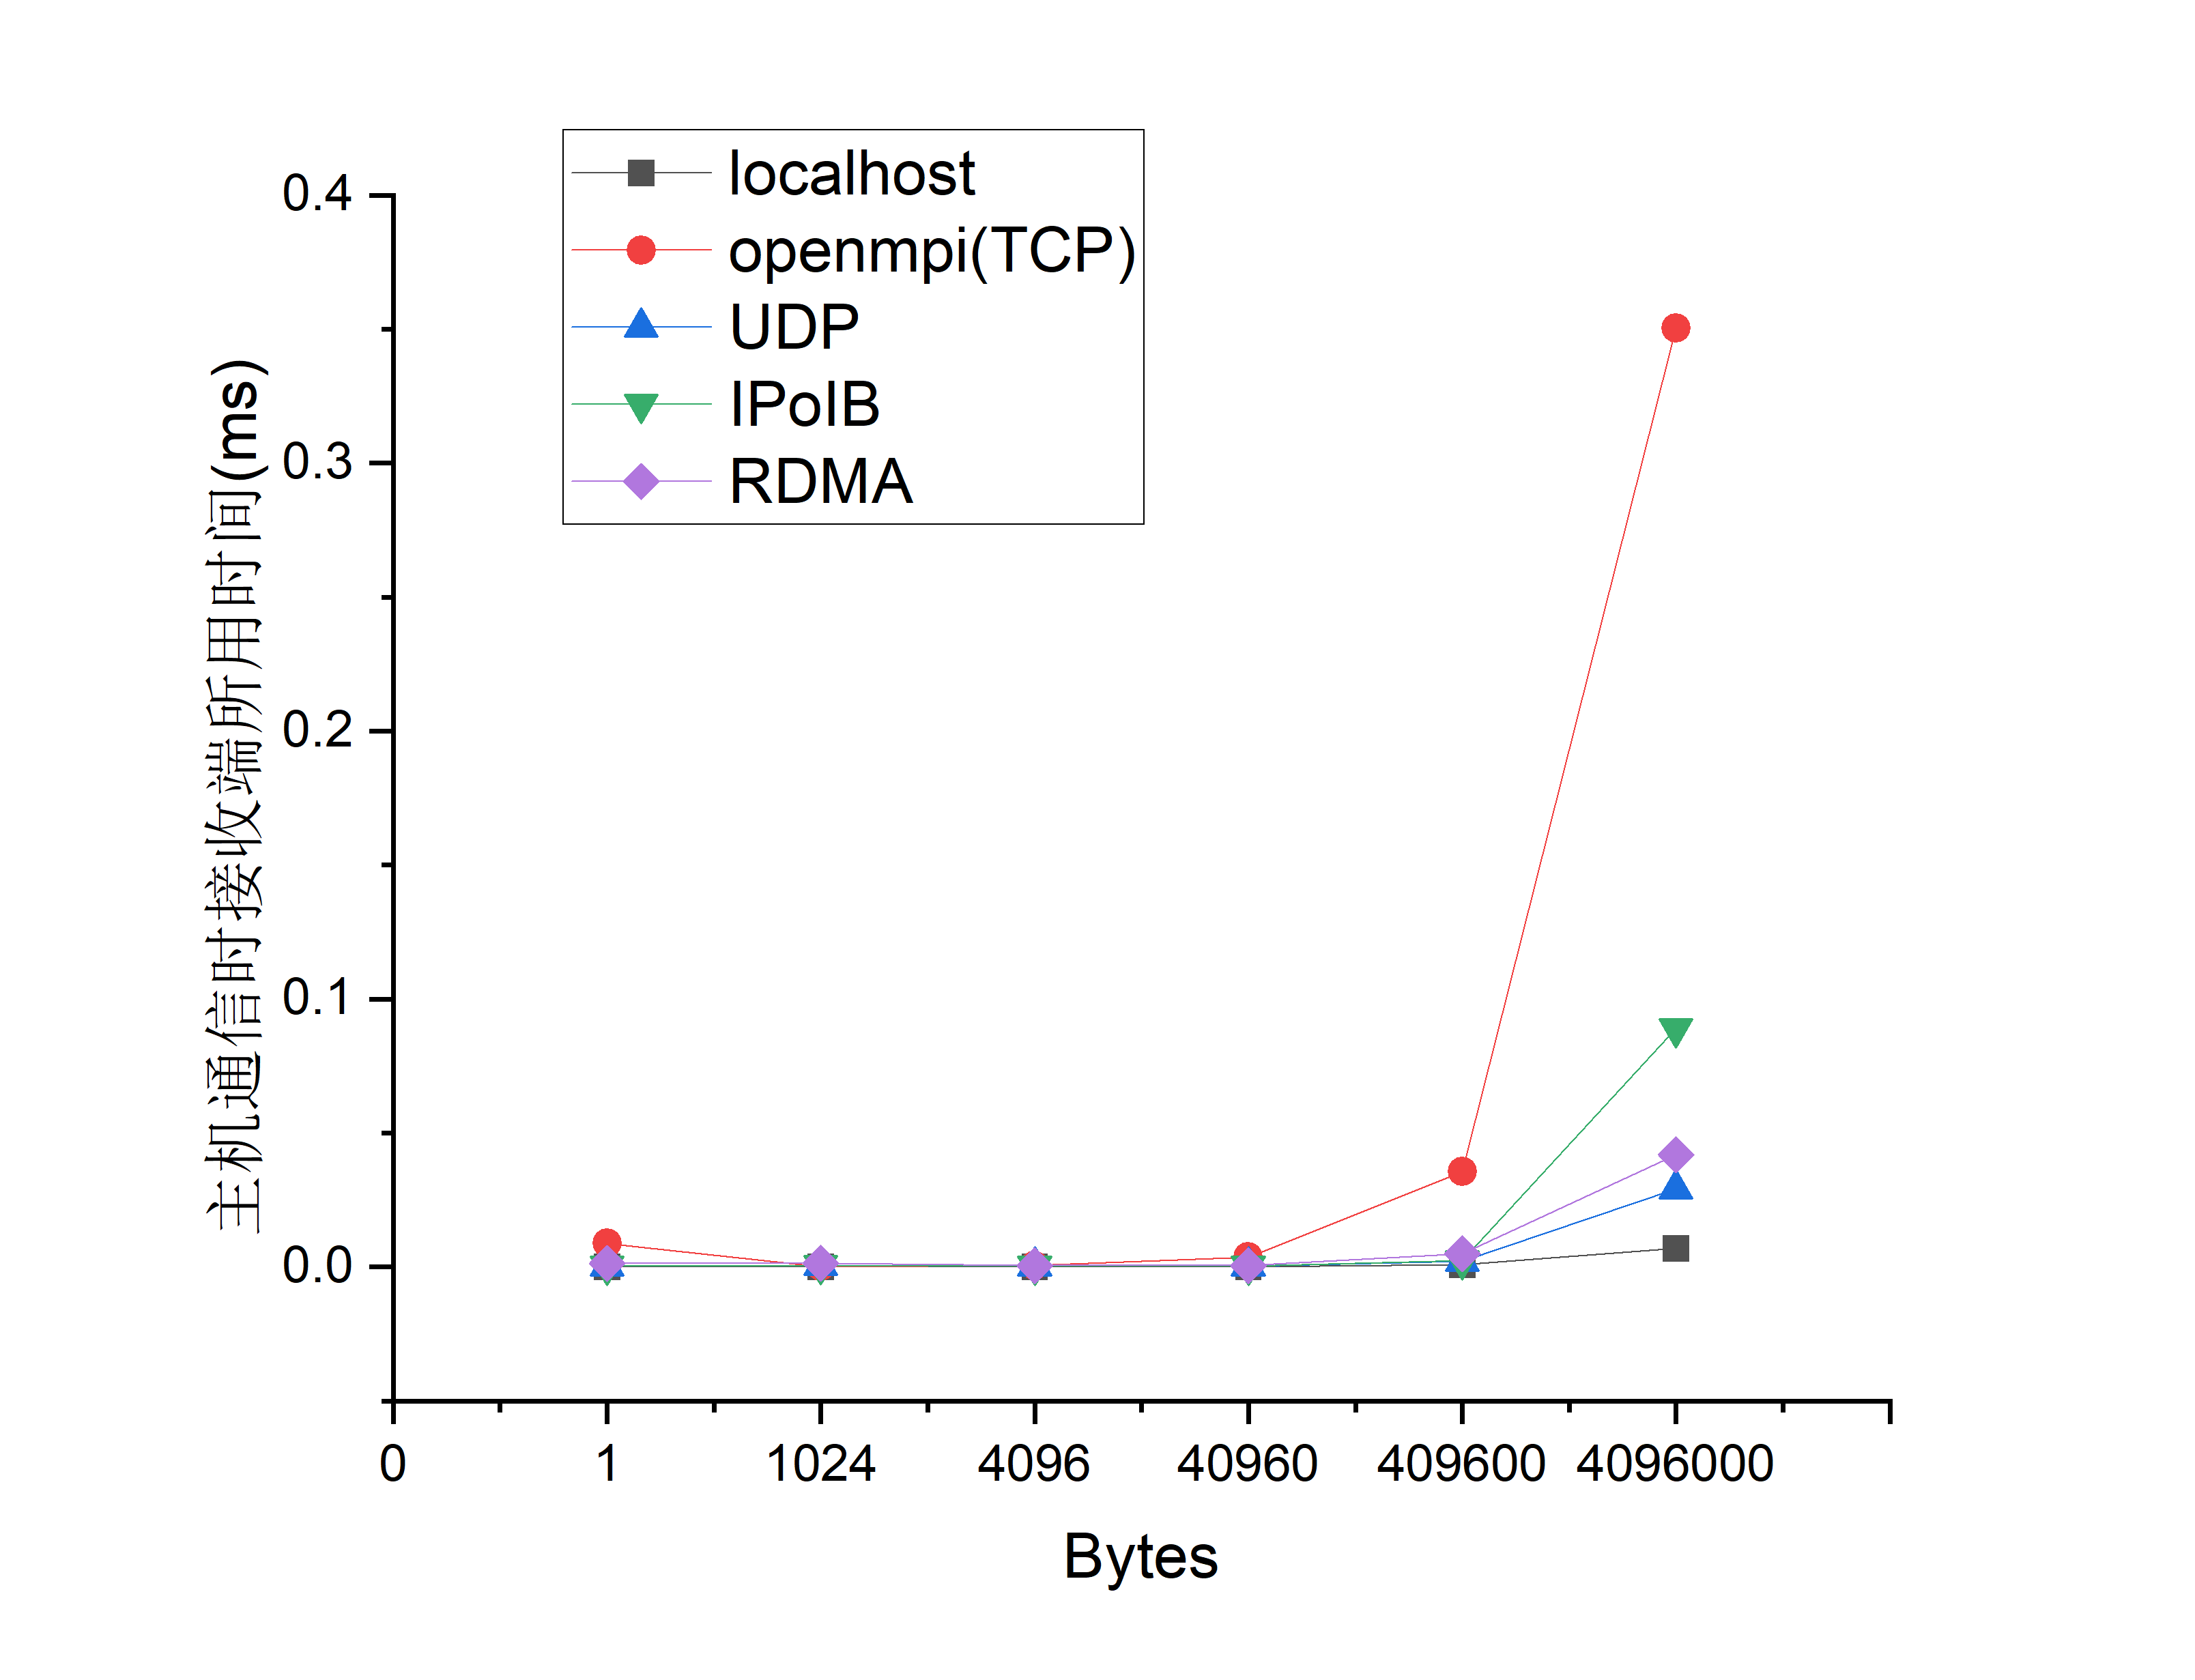
\includegraphics[width=1.0\textwidth]{Img/recv_perf.png}
        \caption{主机不同通信方式花费时间(接收端)}
    \end{figure}

    \begin{figure}[H]
        \centering
        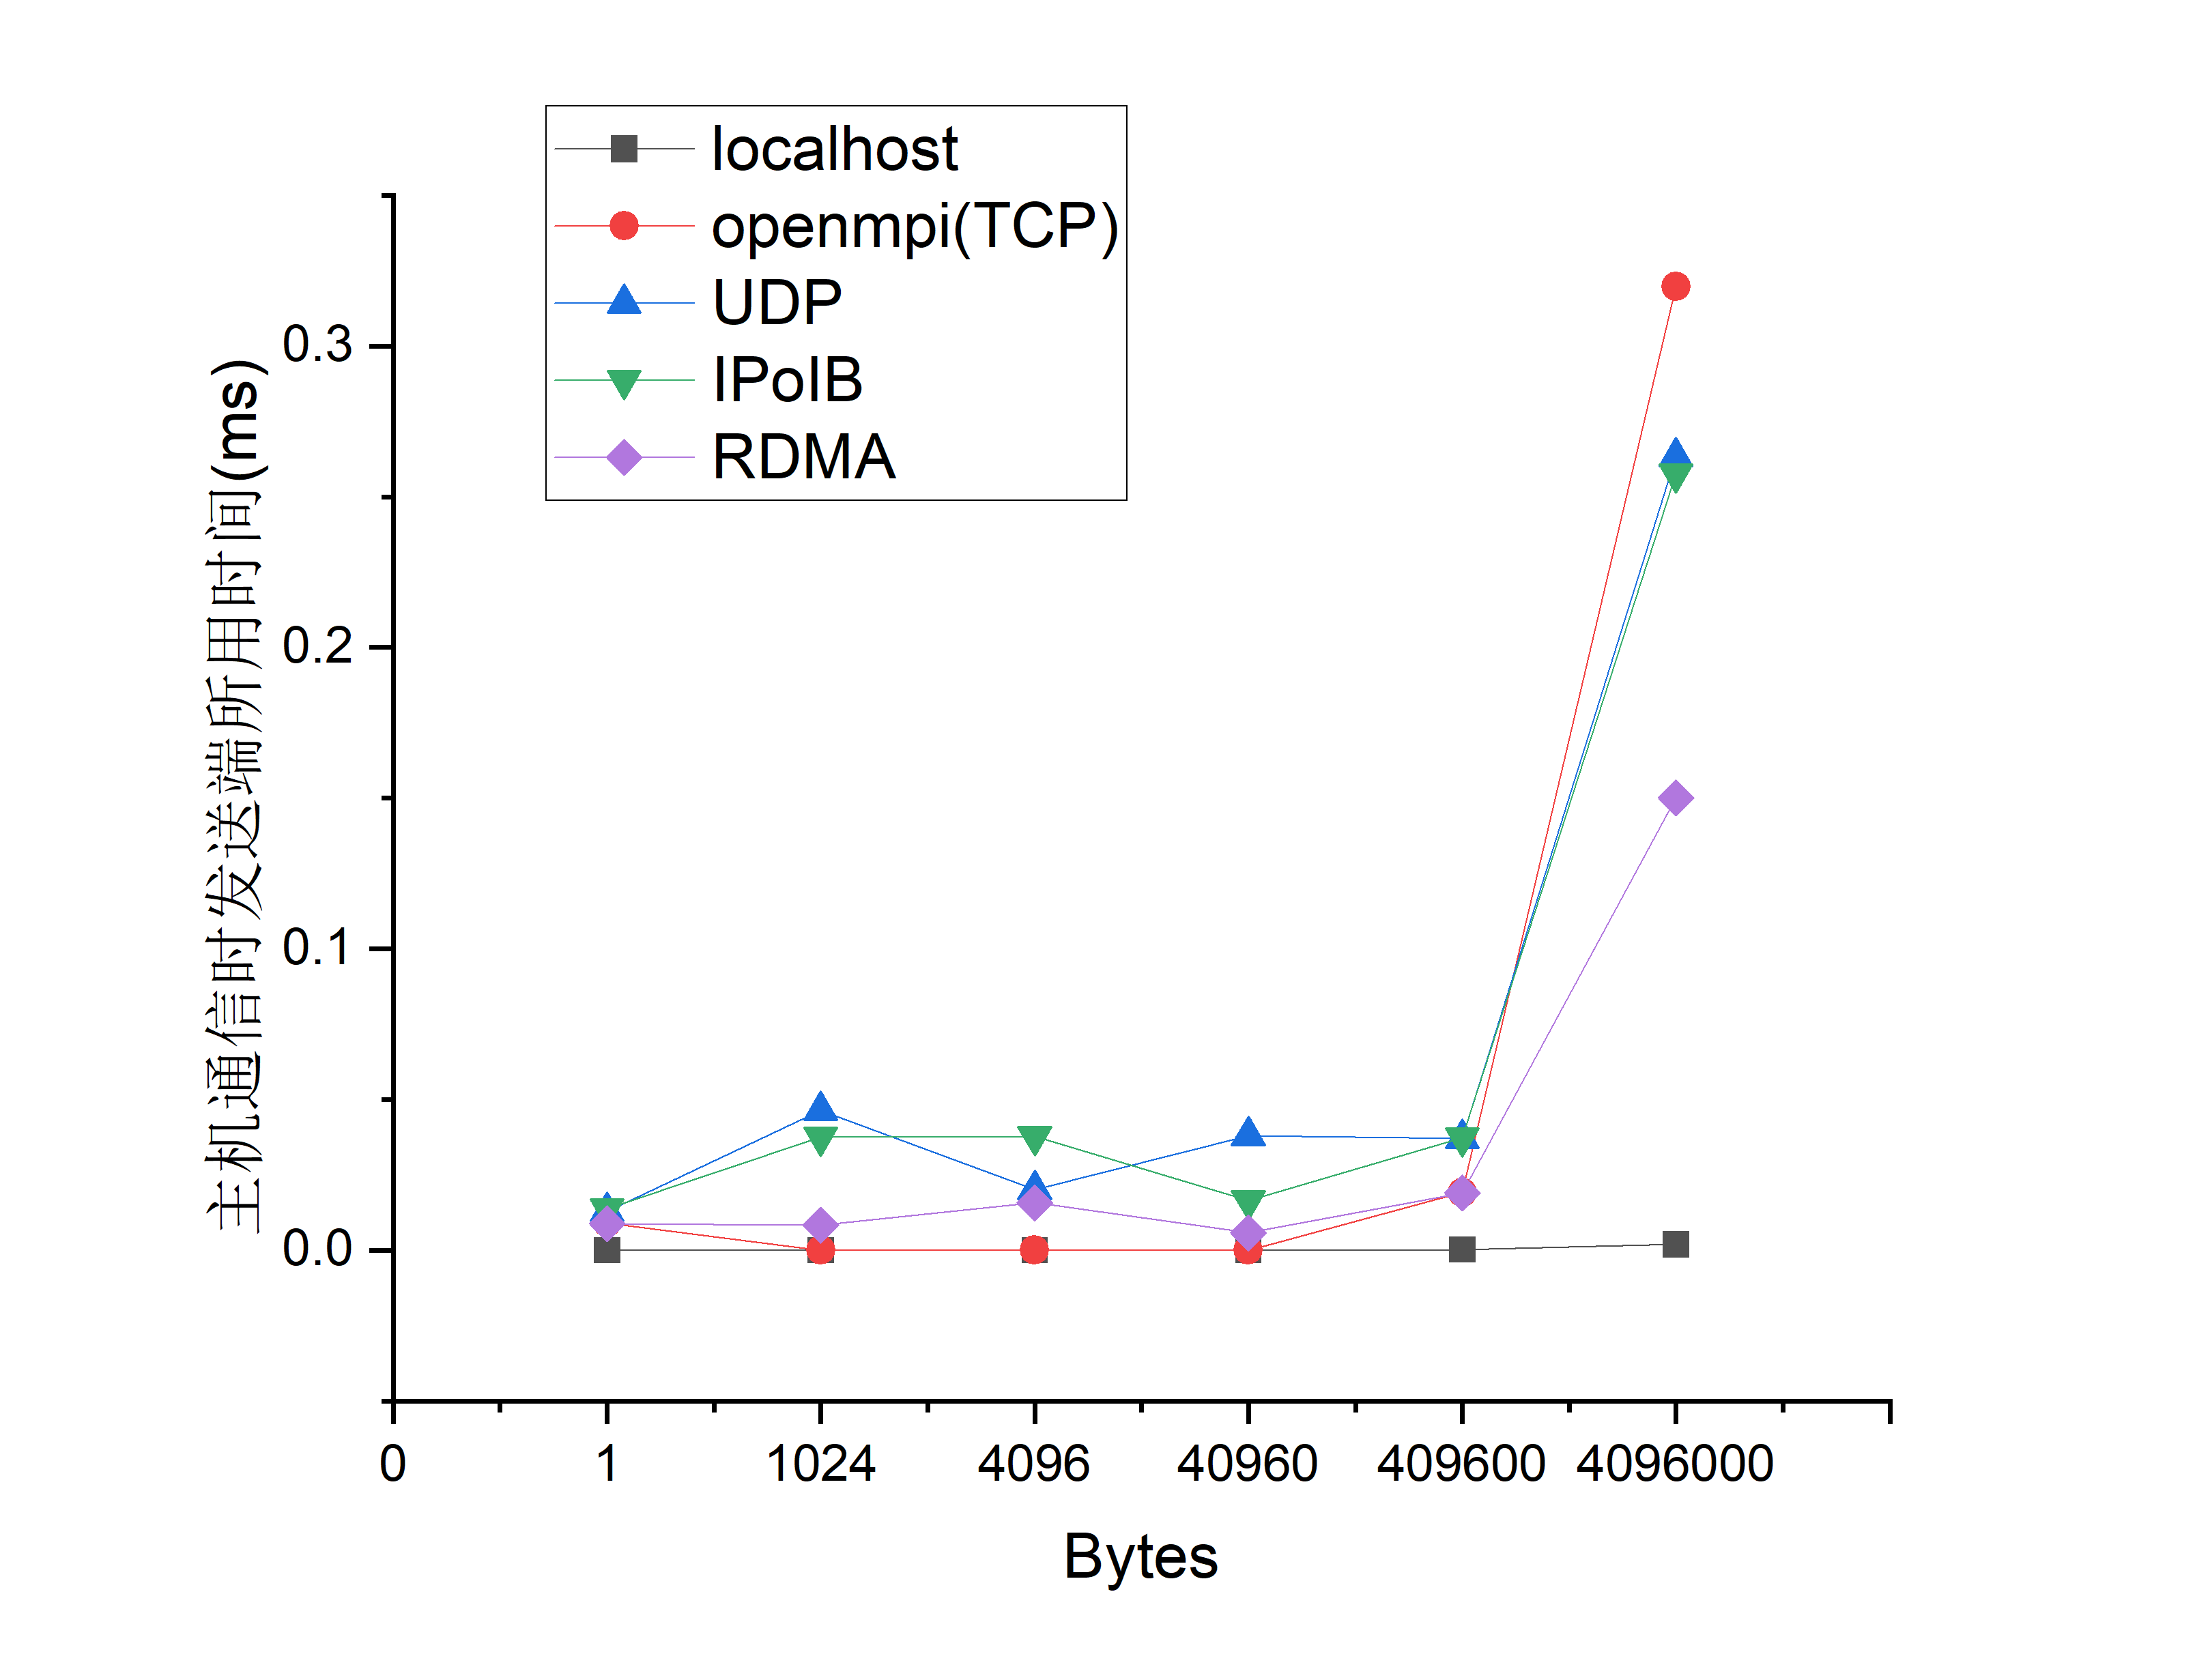
\includegraphics[width=1.0\textwidth]{Img/send_perf.png}
        \caption{主机不同通信方式花费时间(发送端)}
    \end{figure}

    由以上传输字节多少引起的时间变化可以看出
    \begin{itemize}
        \item 接收端四种通信方式在小于40960字节时花费时间大致一致,大于40960字节时TCP连接花费时间显著多于另外三种连接花费时间;同时UDP,IPoIB与RDMA三种连接方式花费时间大致一致,没有显著区别;
        \item 发送端四种通信方式在小于409600字节时花费时间没有显著区别,波动属于正常区间;大于409600字节时TCP,UDP与IPoIB花费时间显著增长,明显多于RDMA发送端花费的时间(约为RDMA花费时间的2倍);
        \item 综合接收端与发送端所花费的时间可以看出,在大文件网络传输的情况下,TCP连接接收端与发送端花费时间均为最长(总时间最长);UDP与IPoIB网络连接总体花费时间大致一致,IpoIB在接收端花费的时间略长一些;RDMA连接花费的时间最短,且在发送端显著低于其他四种连接方式。
    \end{itemize}

    \section{本章小结}
}